\clearpage

\def\chaptertitle{Range Thresholding on Streams}

\lhead{\emph{\chaptertitle}}

\chapter{\chaptertitle}
\label{ch:rts}

\section{Problem Definition}
\label{sec:rts-definition}
We will now formally define the Range Threshold on Streams (RTS) problem. Given a constant integer $d\geq 1$, we consider the \textit{data space} $\mathbb{R}^d$. The \textit{data stream} is an unbounded sequence of elements where the $i$-th $(i\geq1)$ element is denoted as $e_i$ and is said to arrive a time $i$. Each element $e_i$ carries two static fields; $v(e_i)$ - a point in the data space and a weight $w(e_i)\in\mathbb{Z}$. An \textit{RTS query} $q$ specifies a $d$-dimensional axis-parallel rectangle $R_q$ and a given integer threshold $\tau_q$.

If the query is issued after receiving $e_j$ for some $j\geq 1$ then for $t\geq j+1$ we define $S(q,t)$ to represent the elements $e_{j+1},e_{j+2},\dots,e_t$ that \textit{stab} $R_q$. That is, 
$$S(q, t) := \{e_i | j < i \leq t \text{ and } e_i \in R_q\}$$
Define
$$W(q, t) := \sum_{e\in S(q,t)}w(e)$$
Then the \textit{maturity time} of a query $q$ is the smallest $t$ such that $W(q,t)\geq \tau_q$. For a steam of length $n$ (that is, the length of the stream at this point) we will abbrevaiate $S(q,n)$ as $S(q)$ and $W(q, n)$ as $W(q)$.

The RTS problem is to simultaneously support a set of $m$ RTS queries and to correctly report the maturity time of a each query. In addition to managing the maturity of a given set of RTS queries, a solution must also support the following two operations, Register$(q)$: accept a new query at the current moment (after the arrival of $e_n$) and Terminate$(q)$: stop a given query $q$.

\section{Benchmark Solutions}
\label{sec:benchmark-solutions}

The RTS problem is deceptively simple at first glance, given a new stream element $e$ we can check for each query $q$ whether $e \in R_q$ and then increment $W(q)$ accordingly. This algorithm is trivially correct, though results in a quadratic $\Theta(nm)$ computation. Whilst a quadratic runtime appears acceptable, this method becomes intractable when $m$ is large. Our goal therefore, is to devise an algorithm that avoids this \textit{quadratic trap}.

We also emphasis that we are considering an \textit{unbounded} long stream of elements, all solutions explored are restricted to have a memory footprint in terms of $m$, as a Data Structure on the data stream itself is guaranteed to become prohibitively large.

\subsection{Naive Algorithm}
\label{sec:naive-algorithm}

As a simple baseline approach we will formally outline the most naive algorithm for solving the RTS problem:

\begin{algorithm}
\caption{Naive RTS}\label{alg:naive-rts}
\begin{algorithmic}[1]
\Procedure{Naive-RTS}{query set $Q^*$}
\State \text{store query $q$ in an array, along with counters $c_q\gets 0$}
\For{ \text{each stream element $e$}}
\For{ \text{each $q\in Q^*$}}
\State \text{if $e\in R_q$ set $c_q \gets c_q + w(e)$}
\State \text{if $c_q \geq \tau_q$, mature query $q$}
\EndFor
\EndFor
\EndProcedure
\end{algorithmic}
\end{algorithm}

The Register and Terminate operations can also be trivially supported in $O(1)$ time by appending and removing from the array. 

\subsection{Stabbing Data Structures}
\label{sec:stabbing-data-structs}

A number of problems in the Computer Science literature involve the so-called stabbing query

\begin{definition}[Stabbing Query] Given a point $v$ in the data space $\mathbb{R}^d$ report the set of intervals $I$ in some set $Q$ such that $v \in I$. The returned set of queries are set to \textit{stabbed} by $Q$.
\end{definition}

Given its abundance, such operations have been well studied \cite{DBLP:conf/soda/Rahul15}.  Clearly, the RTS problem defined in \cref{sec:rts-definition} is itself a generalised form of stabbing query so existing data structures that support such operations, which can naturally be applied in the context of the RTS problem. We consider some notable examples below. 

\textbf{Interval Trees.}

The Interval Tree \cite{DBLP:books/lib/BergCKO08} is a data structure designed for storing intervals, and efficiently reporting stabbing queries on said intervals. In $d$-dimensional space, the Interval Tree supports $O(1)$ insertion and deletion and performs a stabbing operation in $\Tilde{O}(1 + k)$ time, where $k$ is the number of intervals reported. In terms of space, a $d$-dimensional Interval has a memory footprint of $\Tilde{O}(m)$.

The interval tree can naturally be extended to solve the RTS problem, by maintain a hash-set of counters $c_q$ for each registered interval $R_q$. For an incoming stream element, the interval tree can report all stabbed intervals in $\Tilde{O}(1+k)$ and update counters and report queries in $O(k)$. Although an improvement over the naive approach, in the worst case $k =m$ implying a time complexity of $O(nm)$ to process a stream of length $n$.



\textbf{R Trees.}

\section{DT Algorithm}
\label{sec:DT-algorithm}

As we have seen, all benchmark solutions are unable to escape the quadratic trap in runtime which become impractical for massive values in $m$ and $n$. In this section, we present the state of the art \textit{DT Algorithm} \cite{GAN16}, as well as prove its correctness and sub-quadratic time complexity.

Before diving into how the algorithm is derived, we will first deliver some quick intuition. To escape the quadratic trap of existing solutions, the DT algorithm proposes a tree-based structure to process queries, where the height of the tree is guaranteed to be $O(\log m)$. The tree-structure is designed so that vertices hold a so-called \textit{Jurisdiction Interval}, which corresponds to portions of registered query intervals. A counter is maintained at each vertex, so that as elements are processed, the counter of nodes whose Jurisdiction Interval is stabbed by the value of the stream element is updated by its weight. The \textit{trick} behind the DT Algorithm is to then map queries and vertices to instances of Distributed Tracking, as described in \cref{sec:dist-tracking}. In doing so, the algorithm is able to efficiently report the maturity of queries across the tree. 

\subsection{Constrained RTS Case}
\label{ssec:constrained-DT-algorithm}

For the moment, we restrain the RTS problem in the following ways: Set the dimension of the data space $d = 1$ and assume for each stream element we have $w(e) =1$. Moreover, we enforce that all queries are registered at the beginning, before receiving the first stream element, and no query is allowed to be registered afterwards. We refer to this latter condition as the \textit{one-time registration constraint}.

We will now present and analyse a version of the DT Algorithm for solving this constrained problem, before extending the algorithm to solve the most general version of RTS problem given in \cref{sec:rts-definition}.

\textbf{The Endpoint Tree.} We begin by denoting $Q^*$ as the set of registered RTS queries. The first step of the algorithm is to construct a special binary tree $\mathcal{T}$ on the sorted endpoints of the intervals in $Q^*$. For the remainder of this thesis, any tree constructed this way will be referred to as an \textit{endpoint tree}. For each vertex $v\in V(\mathcal{T})$ we define its \textit{jurisdiction interval} as follows: 

\begin{definition}[Jurisdiction Interval]
    For each $v\in V(\mathcal{T})$ we define the \textit{jurisdiction interval associated with v}, denoted by $I(v)$ as follows. When $v$ is a \textit{leaf node} of $\mathcal{T}$ then $I(v) := [x, x^\prime)$ where $x$ is the endpoint associated with $v$ and $x^\prime$ is the endpoint associated with the leaf succeeding $v$. In the case that $v$ is the rightmost leaf of $\mathcal{T}$ define $x^\prime = +\infty$. When $V$ is not a leaf, define $I(v) := I(v.left) \cup I(v.right)$ where \textit{v.left} and \textit{v.right} denote the left and right child nodes of $v$.
\end{definition} 

\begin{example}
    Consider the following endpoint tree
    \begin{center}
        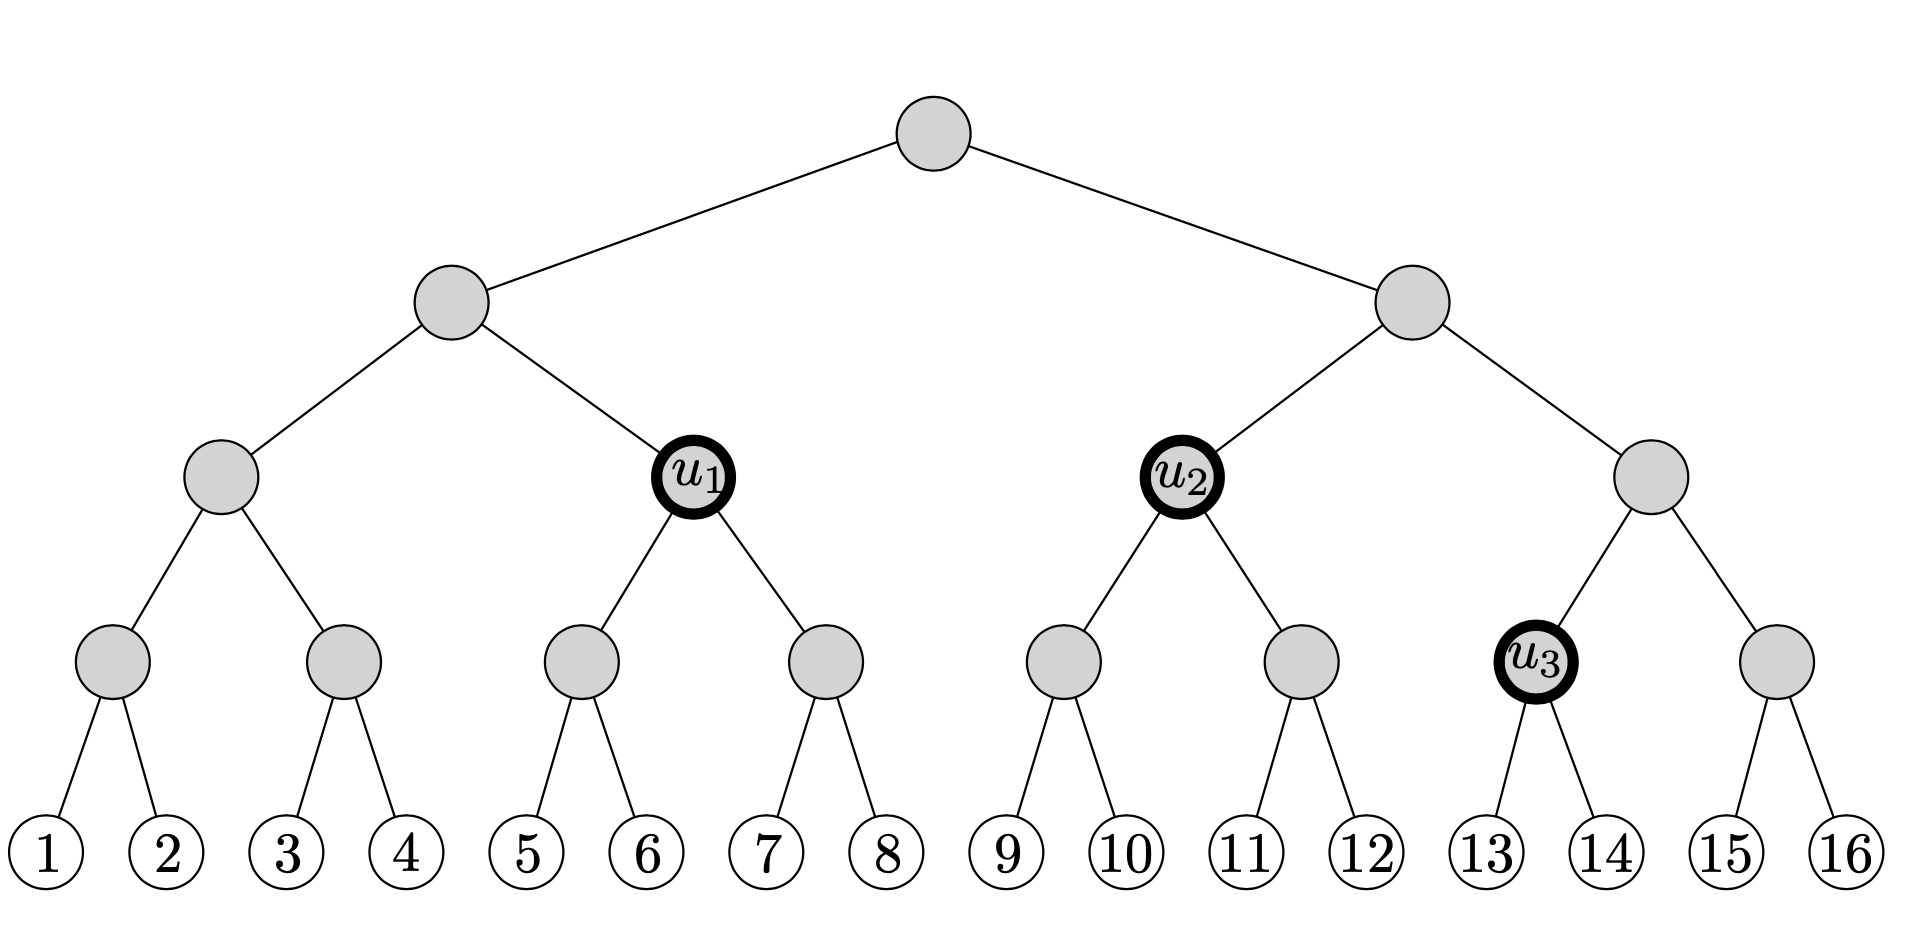
\includegraphics[scale=0.3]{thesis/figures/endpointTree2.png}
    \end{center}
    The jurisdiction interval associated with the node for endpoint 1 is $[1, 2)$. For the other labelled nodes $I(u_1) = [5, 9)$, $I(u_2) = [9, 13)$ and $I(u_3) = [13, 15)$.
\end{example}


In addition to each vertex $v$ having a jurisdiction interval, we also initialise a \textit{count} for each vertex $c(v) \leftarrow 0$. Once the tree has been constructed we now commence the data stream. Let $e$ be an incoming stream element such that $v(e)$ is at least the leftmost endpoint of $\mathcal{T}$ (otherwise, $e$ can be safely ignored). Starting at the root, trace a path to a leaf of $\mathcal{T}$ based on which nodes $u\in V(\mathcal{T})$ satisfy $v(e) \in I(u)$. For each node $u$ that is traced we increment the corresponding counter $c(u) \leftarrow c(u) + 1$. We refer to this procedure as the \textit{element processing} portion of the algorithm and we prove the following claims: 

\begin{lemma} For any stream element $e$ and endpoint tree $\mathcal{T}$, $v(e)$ stabs at most one jurisdiction interval at each level of $\mathcal{T}$. That is, at each level of $\mathcal{T}$, there is precisely one node $u$ such that $v(e)\in I(u)$.
\end{lemma}
\begin{proof}
    By contradiction suppose that $v(e)$ stabs two intervals $I(u_1)$ and $I(u_2)$ at the same level. Then $I(u_1) \cap I(u_2)\neq \emptyset$ which means the right endpoint of $I(u_1)$ must be greater than the left endpoint of $I(u_2)$, which is not possible from the construction of the tree, as nodes where constructed based on sorted order.
\end{proof}

\begin{lemma} For a set of $m$ queries, an endpoint tree $\mathcal{T}$ can be constructed in $O(m\log m)$ time, and element processing requires $O(\log m)$ time for each stream element.
\end{lemma}
\begin{proof}
     $\mathcal{T}$ can be constructed by first sorting the $2m$ endpoints of the query set, then recursively constructing the tree based off of adjacent nodes in a \textit{bottom-up} manner. During the construction of the tree, each vertex's jursdiction interval and counter can be initialised in $O(1)$ time. The runtime is dominated by the sorting which is $O(2m \log 2m) = O(m\log m)$. As the binary tree is built in a \textit{bottom-up} approach, we are guaranteed that the resulting tree is height-balanced, which implies the height is $O(\log m)$. Using Lemma 3.2 we know that we must only consider a single node at level of $\mathcal{T}$, which implies the element processing cost is on the order of the height of the tree which is $O(\log m)$.
\end{proof}

\textbf{Applying Distributed Tracking.} 
We now reveal how nodes in the endpoint tree and their jurisdiction intervals coincide with RTS queries. Then, we will demonstrate how to effectively leverage Distributed Tracking algorithms to efficiently manage query maturation across the endpoint tree. First we require the following definition

\begin{definition}[Canonical Node Set] For a given query $q\in Q^*$ with interval $R_q$ and endpoint tree $\mathcal{T}$ the \textit{Canonical node set} $U_q$ is the smallest $U_q\subseteq V(\mathcal{T})$ such that the jurisdiction intervals of $v\in U_q$ are pairwise disjoint and $R_q = \bigcup_{u\in U_q} I(u)$.
\end{definition}

\begin{example}
    Consider the following endpoint tree built on the query set
    \begin{center}
        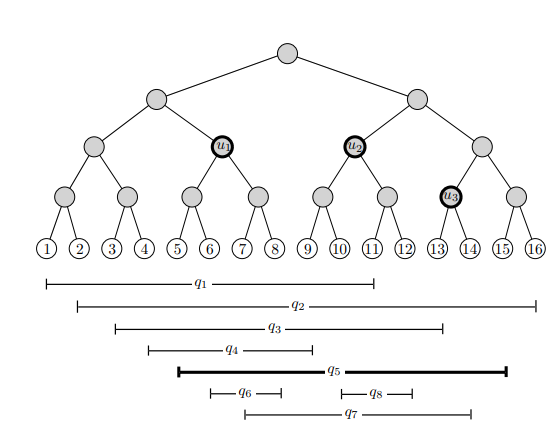
\includegraphics[scale=0.7]{thesis/figures/endpoint_tree.png}
    \end{center}
    For $q_5$ with $R_{q_5} = [5, 15)$ the Canonical Node set $U_{q_5}$ is $\{u_1, u_2, u_3\}$
\end{example}

For a given query $q$ with threshold $\tau_q$ and canonical node set $U_q$ we can consider a conceptual instance of distributed tracking with participants equal to $u\in U_q$, participant counters $c(u)$ as defined in the endpoint tree and the coordinator threshold set to $\tau_q$. In this scenario, we view the query as the coordinator itself, whose mission is to capture the exact instant that 
\begin{equation}
    \tau_q = \sum_{u \in U_q} c(u) = W(q)
\end{equation}
We now execute an instance of \cref{alg:dist-tracking}, simulating each of its steps. We perform the element processing, and update each counter $c(u)$ in $\mathcal{T}$, these correspond to counter increments in \cref{alg:dist-tracking}. When condition $(3.1)$ is met via \cref{alg:dist-tracking}, this corresponds to query maturation in our range thresholding problem. 

As is emphasised in \cite{GAN16}, there is nothing \textit{distributed} in this configuration and all computation runs off of a single CPU. We simply leverage \cref{alg:dist-tracking} to efficiently identify the moment that an RTS query matures. 

Returning to the DT Algorithm, we can determine the canonical node set of each query in $O(\log m)$ time according to the following procedure: 

\begin{algorithm}\label{alg:get-canonical-node-set}
\begin{algorithmic}[1]
\Procedure{GetCanonicalNodeSet}{$q$}
\State \text{Let $x, y$ be the endpoints of $R_q$}
\State \text{Let $z_1, z_2$ be the leaves storing $x,y$ respectively}
\State \text{Identify the lower comment ancestor $u$ of $z_1, z_2$}
\State\text{$U_q \gets$ ADD($u, x, y$)}
\EndProcedure
\State
\Procedure{Add}{$u, x, y$}
\State \text{If $I(u)\subseteq[x,y)$ add $u$ to $U_q$ and \textbf{return}}
\State \text{Else if $I(u)\cap [x,y) = \emptyset$ \textbf{return}}
\State \text{Else ADD$(u_1)$ and ADD($u_2$) where $u_1, u_2$ are children of $u$}
\EndProcedure
\end{algorithmic}
\end{algorithm}

\begin{lemma}[Correctness, Time Complexity]
    For a given RTS query $q$ and endpoint tree $\mathcal{T}$, the above procedure determines the canonical node set $U_q$ in $O(\log m)$ time.
\end{lemma}
\begin{proof} The algorithm is correct, as it only adds nodes whose jurisdiction interval coincides with $R_q$, beginning from the lowest common ancestor (LCA) of the endpoints of $R_q$. By the construction of the endpoint tree, all members of the canonical node set with belong to the subset of nodes of the tree rooted at the LCA $u$ as  $R_q\subseteq I(u)$. Finally, the time to determine the LCA, and the depth of recursion of the ADD procedure is bounded by the height of the tree, which is $O(\log m)$.
\end{proof}

Important to analyse the complexity of the overall DT Algorithm we also require the following lemma to bound the size the Distributed Tracking instances

\begin{lemma}[Size of Canonical Node Sets]
    For a given RTS query $q$ with canonical node set $U_q$ we have $|U_q| = O(\log m)$
\end{lemma}
\begin{proof}
We claim that at each level of the endpoint tree, at most two nodes can belong to $U_q$. To prove this claim, let $u_1, u_2, u_3$ be nodes at the same depth ordered from left to right, and let $p(u)$ be the parent node of a given $u$.  Suppose that $I(u_1)\bigcup I(u_x) = [x, y)$. Note that by construction, all Jurisdiction Intervals at a given level are disjoint and ordered from left to right. We now claim that $p(u_1) = p(u_2)$ or $p(u_2)$ is to the right of $p(u_1)$. In the first case, the rightmost point of $I(p(u_1))$ is the same as the rightmost point of $I(p(u_2))$. In the second case, the rightmost point of $I(p(u_2))$ is to the right of the leftmost point of $I(p(u_1))$ as intervals are disjoint. In either case, we establish that $I(p(u_2))$ begins at, or is to the right of $I(u_1)$'s leftmost point. Symmetrical argument shows that $I(p(u_2))$ ends at, or is to the left of $I(u_3)$'s rightmost point. These two facts combine to give $I(p(u_2))$ being contained in $[x, y)$ and therefore at most two of $\{u_1, u_2, u_3\}$ will be included in the canonical node set.  As this holds for all depths in a tree of height $O(\log m)$ we conclude that $|U_q| = O(\log m)$.
\end{proof}

 As we have seen, each query $q\in Q^*$ defines an instance Distributed Tracking which we solve using \cref{alg:dist-tracking}. Recall from our description of \cref{alg:dist-tracking}, every node $u\in U_q$ maintains a counter $\Bar{c}_q(u)$ at the time of the last signal to the coordinator, $q$. The next signal from $u$ takes place when
\begin{equation}
    c(u) - \Bar{c}_q(u) = \lambda_q
\end{equation}
where $\lambda_q = \left\lfloor \frac{\tau_q}{2 |U_q|}\right\rfloor$ is the slack value described in \cref{alg:dist-tracking}. As part of the distributed tracking algorithm, the node $u$ needs to inspect condition (3.2) whenever $c(u)$ is incremented. By lemma 3.3 this implies $O(\log m)$ slack inspections per element processing. Theorem 2.5 gives the total messaging cost per query as $O(|U|_q\log \tau_q) = O(\log m\log\tau_q)$ by lemma 3.6.

\textbf{Organising Queries with Heaps.} The steps taken so far seem promising to result in a sub-quadratic algorithm, however let's pay close attention to the cost of inspecting the slack condition (3.2). For a given node $u\in V(\mathcal{T})$, let $Q(u)$ be the set set of queries that have $u$ in their canonical node set. Suppose that $c(u)$ has just been incremented, and we must now inspect condition (3.2). if done naively, one would need to check condition $(3.2)$ for each $q\in Q(u)$. Clearly, this would require $O(|Q(u)|) = O(m)$ time, which coupled with $O(n\log m)$ element processing time for a stream of size $n$ would deprecate the performance of the algorithm to a quadratic $O(nm\log m)$.

Fortunately, with a few observations we can leverage the Min-Heap described in \cref{sec:heap-data-structs} to avoid this. The idea is to inspect only \textit{one} slack condition in $Q(u)$, instead of all $|Q(u)|$. To see how one can do this, define for each $q$ the \textit{key}-value of 
\begin{equation}
    \sigma_q(u) := \lambda_q + \Bar{c}_q(u)
\end{equation}
where $\lambda_q, \Bar{c}_q$ correspond to values defined by \cref{alg:dist-tracking}. Intuitively $\sigma_q(u)$ represents the \textit{next} value of $c_q(u)$ for when the next signal from node $u$ to its coordinator $q$ should occur. The key observation is that, for $q_1, q_2 \in Q(u)$ with $\sigma_{q_{1}}(u) < \sigma_{q_{2}}(u)$ then $c_{q_1}(u) < c_{q_2}(u)$. That is, if we don't need to send a message for $q_1$, then we can immediately deduce that we do not need to send a messages for $q_2$. Using this key observation, the algorithm maintains a Min-Heap $\mathcal{H}(u)$ on $Q(u)$ for each $u\in V(\mathcal{T})$ and applies the following procedure whenever a counter is incremented.

\begin{algorithm}\label{alg:slack-inspection}
\begin{algorithmic}[1]
\Procedure{SlackInspection}{$u$}
\State \text{Find the minimum $\sigma_q(u)$ in $\mathcal{H}(u)$}
\State \text{If $\sigma_q(u) < c(u)$, then we are done.}
\State \text{Otherwise, remove $\sigma_q(u)$ from       
             $\mathcal{H}(u)$. }
\Statex \text{\hspace{5mm} Instruct $u$ to send a signal to $q$ as per \cref{alg:dist-tracking}}
\Statex \text{\hspace{5mm} \textbf{return} SlackInspection$(u)$}
\Comment{Recursive call}
\EndProcedure
\end{algorithmic}
\end{algorithm}

Using the SlackInspection procedure, we can now bound the time required to manage Distributed Tracking related messages over the course of the algorithm:

\begin{lemma}[Slack Inspection Time Complexity]
    The total number of Distributed Tracking signals sent over the course of length $n$ data stream is $O(n\log m +m\log^2m\log\tau_{\max})$
\end{lemma}
\begin{proof}
    Distributed Tracking signals can only be sent via line 4 of the Slack Inspection procedure. It is clear that the SlackInspection procedure runs in 
\begin{equation}
    O(1 + x\log m)
\end{equation}
time, where $x$ is the number of recursive calls made in step 4. Whilst it is almost to bound $x$ in (3.4) for any given iteration, we can instead derive a bound for the entire course of processing a data stream. 

The $O(1)$ term in (3.4) occurs $O(n\log m)$ times, because each stream element can increase the counters of $O(\log m)$ nodes. To bound the $x$ component, notice that the total number of signals sent over the course of the algorithm is 
\begin{align*}
  \sum_{q\in Q^*}O(h_q \log \tau_q) &= \sum_{q\in Q^*} O(|U_q|\log\tau_q) \\
  &= \sum_{q\in Q^*} O(\log m\log\tau_q) \hspace{10mm} \text{(lemma 3.7)} \\
  &= O(m\log m\log\tau_{\max})
\end{align*}
Therefore, the time complexity of all slack inspections over the course of the data stream described by (3.4) can be bounded by $O(n\log m + m\log^2m\log\tau_{\max})$

Finally, when a query $q$ matures, the algorithm removes its entry from all heaps $\mathcal{H}(u)$ for all $u\in U_q$. Recall from \cref{sec:heap-data-structs} that removal from min heaps requires $O(\log m)$, this procedure requires a total of $O(|U_q| \log m) = O(\log^2m)$ time. 
\end{proof}

\textbf{Handling Matured Queries.} We now consider the space complexity of the DT algorithm, recalling that the aim is to use $\Tilde{O}(m)$ space at all times. 

Initially, the endpoint tree occupies $\Tilde{O}(m)$ space, which may become wasteful when many queries mature and $m_{\text{alive}}\ll m$. To deal with this issue, the DT algorithm applies a \textit{global rebuilding} procedure which is called after each query is matured: 

\begin{algorithm}\label{alg:global-algoritm}
\begin{algorithmic}[1]
\Procedure{GlobalRebuilding}{}
\State $\text{load}\gets m_{\text{alive}}/m$ 
\State $\text{if load > 1/2 \textbf{return}}$
\State $\text{else for each $q\in Q^*$ alive set }  \tau_q \gets \tau_q-W(q)$
\State $\text{rebuild $\mathcal{T}$ on alive queries in $Q^*$}$
\EndProcedure
\end{algorithmic}
\end{algorithm}

That is, when $m_{\text{alive}} $ has decreased to $m/2$, the entire endpoint tree is destroyed and rebuilt on the alive queries. To ensure correctness, line $4$ of the procedure dictates that we collect all node counters, and reduce the threshold of each alive query to: $\tau_q - \sum_{u\in U_q} c(u)$, effectively ensuring that currently processed stream elements are accounted for in the new structure.

Whilst GlobalRebuilding maintains a promise on the space consumption of the algorithm, we must also consider the additional demands it has on runtime. Fortunately, the operation is not too expensive, and can be further amortised over the life of the algorithm.

\begin{lemma}[Global Rebuilding Time Complexity]
    GlobalRebuilding has an amortised time complexity of $O(m\log m)$ over the course of the entire algorithm
\end{lemma}
\begin{proof}
    Line 4 of the algorithm requires we compute $W(q) = \sum_{u\in U_q}c(u)$ for all $O(m/2)$ alive queries, which by lemma 3.7, requires $O(m\log m)$. Moreover, rebuilding $\mathcal{T}$ is most expensive $O(m/2\log m/2) = O(m\log m)$ time also. To \textit{amortise} the cost of the procedure, we can charge $O(\log m)$ time to mature each query. As each maturity happens only once, the total rebuilding cost is an amortised $O(m\log m)$ for the entire algorithm.
\end{proof}

\textbf{Terminations.} Although for now we enforce the one-time registration constraint, the DT algorithm proposes a simple procedure for implementing a termination.

\begin{algorithm}\label{alg:global-algoritm}
\begin{algorithmic}[1]
\Procedure{Terminate}{$q$}
\State $q.alive\gets false$
\State $\text{delete distributed tracking instance associated with $q$ and}$
\Statex $\hspace{6mm}\text{remove from $\mathcal{H}(u)$ for all $u\in U_q$}$
\EndProcedure
\end{algorithmic}
\end{algorithm}

The bulk of the runtime comes from the removal from the $O(\log m)$ heaps, which from \cref{sec:heap-data-structs}, requires $O(\log m)$. This brings the total time for a Terminate operation to $O(\log ^2 m)$.

A far simpler approach is to simply mark the distributed tracking instance as deleted, and then enhance the SlackInspection procedure to check that the popped minimum corresponds to a \textit{live} Distributed Tracking instance. Doing so avoids the complication of deleting from heaps, and results in a $O(1)$ operation.

\textbf{Analysis.} We have now motivated and explained each component of the DT algorithm. Expressed in psuedo-code, the algorithm for the constrained RTS problem can be described in psuedo code as follows:

\begin{algorithm}
\caption{Constrained DT}\label{alg:constrained-dt}
\begin{algorithmic}[1]
\Require $Q^* \gets m$ \text{ RTS queries $(R_q, \tau_q)$}
\State \text{Build end point tree $\mathcal{T}$ from endpoints in $Q^*$}
\For{ $q \in Q^*$}
    \State \text{Find canonical node set $U_q$}
    \State \text{Create instance of \cref{alg:dist-tracking} on $U_q$}
\EndFor
\State \text{Commence data stream} 
\For{$e_t$ for $t = 1,2,\dots$}
\State \text{Trace $e_t$ through $\mathcal{T}$ based on Jurisdiction Interval}
\State \text{Update node counters $c(v) \gets c(v)+1$ for each $v\in V(\mathcal{T})$ traced}
\State \text{Perform SlackInspection$(v)$ for each $v\in V(\mathcal{T})$ traced}
\State \text{Perform GlobalRebuild()}
\EndFor
\end{algorithmic}
\end{algorithm}

\begin{theorem}[Correctness] The Constrained DT algorithm solves the constrained RTS problem. That is, for each query $q$ the constrained DT algorithm correctly reports the instant that $W(q) = \tau_q$
\end{theorem}
\begin{proof}
    Each $q \in Q^*$ is mapped to an instance of Distributed Tracking which is then solved by \cref{alg:dist-tracking}. The correctness of reporting when $W(q) = \tau_q$ follows as a consequence of Theorem 2.5.
\end{proof}

\begin{theorem}[Time Complexity] For a collection of $m$ RTS queries the constrained DT algorithm requires $O(n\log m + m\log^2m\log\tau_{max})$ time to process a stream of length $n$.
\end{theorem}
\begin{proof}
    The time complexity is simply the combinations of all the components of the algorithm discussed. By Lemma 3.4, constructing the tree and processing elements demands $O(m\log m)$ and $O(n\log m)$ respectively. By Lemma 3.6, determining the Canonical node sets requires $O(m\log m)$, and Lemma 3.9 bounds the global rebuilding procedure as $O(m\log m)$ also. Finally, Lemma 3.8 bounds the total time for processing counter updates and performing slack inspection as $O(n\log m + m\log^2\log m)$ for a stream of length $n$. Summing each of these, the total time is dominated by $O(n\log m + m\log^2m\log\tau_{max})$.
\end{proof}

\begin{theorem}[Space Complexity]
    At all times the DT Algorithm uses $\Tilde{O}(m_{\text{alive}})$ space.
\end{theorem}
\begin{proof}
    If $Q^*$ is the set of alive queries at the time of Reconstruction, then line 3 of the GlobalRebuilding procedure ensures that $m_{\text{alive}}\geq |Q^*|/2$ implying the space consumption is now $O(|Q^*|\log |Q^*|) = O(m_{\text{alive}}\log m_{\text{alive}}) = \Tilde{O}(m_{\text{alive}})$.
\end{proof}

A useful observation is that the runtime of the DT algorithm can be decomposed into the runtime of the \textit{element processing} (tracing a stream element through the endpoint tree) and the runtime of the \textit{communication cost} (the simulated messaging of \cref{alg:dist-tracking}). That is, 
$$O(\underbrace{n\log m}_{\text{element processing}} + \underbrace{m\log ^2 m\log\tau_{max}}_{\text{communication}})$$


\subsection{Unconstrained RTS Case}
\label{ssec:unconstrained-DT-algorithm}

We now reveal how \cref{alg:constrained-dt} can be extended to solve the full, unconstrained RTS problem. We will remove each constraint separately before revealing the complete algorithm. 

\textbf{Enabling Insertions.} The first constraint we will eliminate is the one-time registration condition; that is, will define how to incorporate a Register($q$) procedure for a new RTS query $q$. 

The solution is to apply \textit{Logarithmic Rebuilding} described in \cref{sec:logarithmic-rebuilding}. The query set $Q^*$ is now partitioned into sets $S_1,\dots, S_h$ such that $h = O(\log m)$, each query set $S_i$ contains either $2^i$ queries, or is empty. Importantly, each query belongs to precisely one $S_i$. Associated to each query set is an independent end-point tree $\mathcal{T}_1\dots, \mathcal{T}_h$, built on the endpoints of queries in $S_1,\dots,S_h$. Registering a new query is as described in \cref{sec:logarithmic-rebuilding}, identify the smallest $j$ such that $S_j = \emptyset$ and set $S_j = \bigcup_{i=1}^{j-1}S_i$ along with the new query $q$, and then create a new endpoint tree $\mathcal{T}$ on $S_j$. From Theorem 2.5, this gives us the the cost of the insertion as an amortised $O(m\log^2 m)$.

To preserve the correctness of our original algorithm, given an incoming element $e$ we must now trace it through each $\mathcal{T}_1,\dots,\mathcal{T}_h$. As $h = O(\log m)$ and the height of each tree is $O(\log m)$ this implies an element processing cost of $O(n\log ^2 m)$ for a stream of length $n$. No other details of the algorithm are changed - implying the runtime is now bought to $O(n\log^2m + m\log^2m\log\tau_{\max})$.

\textbf{Multidimensional Queries.} 
To scale to multidimensional queries, the DT Algorithm borrows a technique used by another common Data Structure for computational geometry problems known as \textit{Range Trees }\cite{RangeTrees}. The idea is to recursively \textit{embed} secondary endpoint trees  into nodes of the first endpoint tree. The usual root-to-leaf path tracing for element processing is maintained, though is now performed on these secondary subtrees also. We describe this procedure rigourously in the sections below.

For now, suppose $d=2$ and let $Q^*$ denote the set of all queries. For each $q\in Q^*$, $R_q$ now corresponds to an \textit{axis-parallel rectangle} of the form $R_q = [x, x^\prime) \times [y, y^\prime)$. We will use the notations $R_q(x)$ and $R_q(y)$ to denote the $x$ and $y$ axis components of the rectangle respectively. 

To solve the RTS problem in this setting the DT Algorithm proceeds as before by building an endpoint tree on the endpoints of $R_q(x)$ for each $q\in Q^*$. As before, each query also corresponds to an instance of the \textit{Distributed Tracking} problem with an $x$-canonical node set. Focus on a specific $u\in V(\mathcal{T})$ and denote by $Q(u)$ the set of queries that contain $u$ in their canonical node sets. To extend to $d=2$ queries, we now associate $u$ with a secondary endpoint tree $\mathcal{T}(u)$, built on the endpoints of each $R_q(y)$ in $Q(u)$. 

\begin{figure}[h]
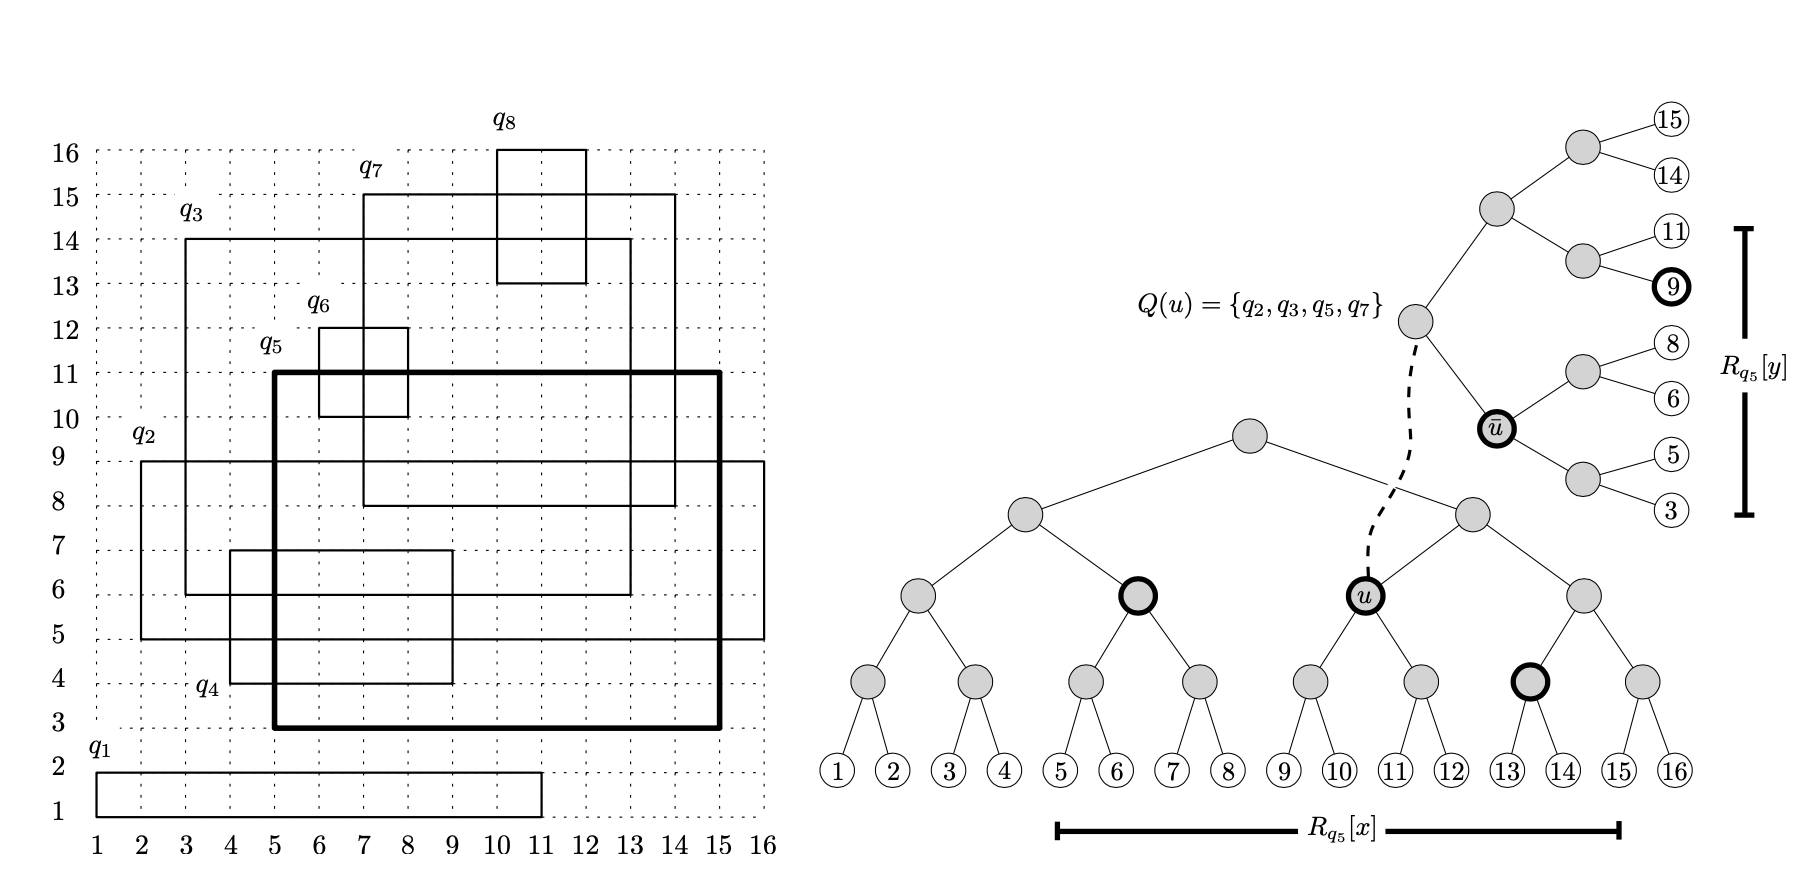
\includegraphics[scale=0.5]{thesis/figures/multdimexample.png}
\caption{An example of $d=2$ Endpoint Tree}
\end{figure}

$\mathcal{T}$ and all the $\mathcal{T}(u)$ now constitute a two dimensional endpoint tree. With an application of Lemma 3.4, such a tree can be constructed in $O(m\log m)$. The \textit{canonical node set} of a given query $U_q$ is now the union of its canonical node set in the $R_q(x)$-endpoint tree and Canonical node set in all $\mathcal{T}(u)$ endpoint trees. Unlike in the $d=1$ case, $|U_q|$ is now $O(\log^2m)$, as the size of any node set in $\mathcal{T}(u)$ is $O(\log m)$ and there is at most $O(\log m)$ of them.

To support element processing of multi-dimensional queries, the algorithm is largely unchaged: First trace a root-to-leaf path $\mathcal{P} $ in $\mathcal{T}$, and then further root-leaf paths in  $\mathcal{T}(u)$ for each $u\in\mathcal{P}$. As before, the DT Algorithm increments the counter of each node visited throughout this process. It is clear each secondary tree has height $O(\log m)$ so this process requires $O(n\log^2m)$ for a stream of length $n$.

The remainder of the algorithm follows exactly as described in \cref{ssec:constrained-DT-algorithm}. As the size of each $U_q$ now becomes $O(\log^2m)$, the total cost of all heap updates given by Lemma 3.8 now becomes $O(m\log^3m\log\tau_{\max})$. Recalling that the logarithmic rebuilding technique adds an additional $\log m$ factor to the element processing cost, the time complexity for $d=2$ queries is now bought to 
$$O(n\log^3m + m\log^3m\log\tau_{\max})$$
effectively adding a logarithmic factor to both terms of the time complexity in the unconstrained case. Range Trees \cite{RangeTrees, DBLP:books/lib/BergCKO08} describe how this method can generalised to $d$-dimensional sapce, by further layering sub trees. It is well known that each additional dimension incurs an extra logarithmic factor to both the running time and space consumption. This brings the total time complexity to $O(n\log^{d+1}m + m\log^{d+1}m\log\tau_{\max})$ and space complexity to $O(m_{\text{alive}}\log^d m_{\text{alive}})$.


\textbf{Weighted Stream Elements.} The final constraint to remove is the restriction on stream weights. To achieve this, we will require a more general Distributed Tracking algorithm which allows for counter updates to be of the form $c(u) \gets c(u) + w$ with $w\in\mathbb{Z}$. 

The straight-forward approach is to just apply \cref{alg:dist-tracking}, though now simply transmit $w$ signals in line 9, one at a time. The drawback of this approach however is that each transmission requires $O(1)$ time which implies the total work of the algorithm becomes $O(\tau + h\log\tau)$, which can become substantially higher than the desired $O(n + h\log\tau)$ if $\tau\gg n$. In turn, this would result in prohibitively high communication cost if substituted into the DT algorithm. 

To handle this problem \cite{GAN16} proposes the following algorithm, which is very close to what is described in \cref{sec:dist-tracking}, though now includes a central \textit{while} loop to manage weighted counter increments. 

\begin{algorithm}
\caption{Efficient Weighted Distributed Tracking}\label{alg:weighted-dist-tracking}
\begin{algorithmic}[1]
\Procedure{WeightedDistributedTracking}{$\tau$, participants $S_1,\dots,S_h$}
\If{$\tau\leq6h$}
    \State \text{Commence brute-force algorithm by sending $O(\tau) = O(h)$ messages}
\EndIf
\State \text{Assign to each participant \textit{slack}} $\lambda \leftarrow \lfloor \tau/2h\rfloor$
\State \text{Assign to each participant $\bar{c}_i\gets0$}
\For{\text{each timestamp}}
\While{$c_i - \bar{c}_i = \lambda$}
    \State \text{$S_i$ transmits signal to $q$}
    \State $\bar{c}_i\gets\bar{c}_i+\lambda$
    \If{$q$ collects $h$ notifications}
        \State $\tau^\prime \gets \tau - \sum_{i=1}^{h}c_i$
        \State \textbf{return} \text{DistributedTracking}$(\tau^\prime, S_1,\dots,S_h)$ \Comment{recursive call}
\EndProcedure
\end{algorithmic}
\end{algorithm}

The algorithm is correct as if the round has still not ended at the end of a given time stamp then
\begin{align*}
    \sum_{i=1}^{h}c_i\leq \lambda(h-1) + \sum_{i=1}^{h}(c_i - \bar{c}_i) 
    &<2\lambda h \\
    &\leq\tau
\end{align*}
As argued in \cref{sec:dist-tracking}, the number of rounds is still $O(\log\tau)$, implying the total number of messages remains $O(h\log\tau)$. The addition of line 8 however implies the computation time of the new algorithm is now $O(n + h\log\tau)$.

\textbf{Final Algorithm.} The final DT Algorirthm is exactly as described in \cref{alg:constrained-dt}, though now with the Distributed Tracking algorithm described by \cref{alg:weighted-dist-tracking}, and the multidimensional trees described earlier. Similarly, the Register$(q)$ is handled as discussed. This brings us to the main theorem presented in \cite{GAN16}, whose proof is a culmination of all the results discussed in this section. 

\begin{theorem}[DT Algorirthm Time and Space Complexity]
    The DT Algorithm solves the $d$-dimensional RTS problem in time $O(n\log^{d+1}m + m\log^{d+1}\log\tau_{\max})$ time and  $O(m_{\text{alive}}\log^d m_{\text{alive}})$ space. 
\end{theorem}
